% Template for Elsevier CRC journal article
% version 1.1-5p dated 18 January 2011
% SEM ACENTUACAO PROBLEMA UTF-8 : NAO ACEITA

% This file (c) 2010-2011 Elsevier Ltd.  Modifications may be freely made,
% provided the edited file is saved under a different name

% This file contains modifications for Procedia Computer Science
% but may easily be adapted to other journals

% Changes since version 1.0
% - elsarticle class option changed from 1p to 3p (to better reflect CRC layout)
% - this version uses option 5p for larger-format journals (text area 24.1 x 18.4 cm)

%-----------------------------------------------------------------------------------

%% This template uses the elsarticle.cls document class and the extension package ecrc.sty
%% For full documentation on usage of elsarticle.cls, consult the documentation "elsdoc.pdf"
%% Further resources available at http://www.elsevier.com/latex

%-----------------------------------------------------------------------------------

%%%%%%%%%%%%%%%%%%%%%%%%%%%%%%%%%%%%%%%%%%%%%%
%%%%%%%%%%%%%%%%%%%%%%%%%%%%%%%%%%%%%%%%%%%%%%
%%                                          %%
%% Important note on usage                  %%
%% -----------------------                  %%
%% This file must be compiled with PDFLaTeX %%
%% Using standard LaTeX will not work!      %%
%%                                          %%
%%%%%%%%%%%%%%%%%%%%%%%%%%%%%%%%%%%%%%%%%%%%%%
%%%%%%%%%%%%%%%%%%%%%%%%%%%%%%%%%%%%%%%%%%%%%%

%% The '5p' and 'times' class options of elsarticle are used for Elsevier CRC
\documentclass[1p,times,authoryear]{elsarticle}

%% The `ecrc' package must be called to make the CRC functionality available
%% ecrc_RIAI es el paquete ecrc de Elsevier con modificaciones para la revista RIAI
% \usepackage{ecrc_RIAI}

%% The ecrc package defines commands needed for running heads and logos.
%% For running heads, you can set the journal name, the volume, the starting page and the authors

%%%%%%%%%%%%%%%%%%%%%%%%%%%%%%%%% Aaadido por Secretaraa RIAI
% \usepackage[spanish]{babel}     % Idioma
% \addto\captionsspanish{%
% \def\tablename{Tabla}%
% }
\usepackage{tikz}
\usepackage{algpseudocode}
\usepackage{amsmath}
\usepackage[latin1]{inputenc}   % Lengua latina
\usepackage{amsmath}            % Para las referencias a ecuaciones con \eqref
\usepackage{epstopdf}           % Para poder insertar figuras .eps al compilar con PDFLATEX
\usepackage{flushend}           % Para igualar las columnas de la altima pagina
%\usepackage{hyperref}           % Para hipervanculos dentro del PDF
%%%%%%%%%%%%%%%%%%%%%%%%%%%%%%%%%%%%%%%%%%%%%%%%%%%%%%%


%% set the volume if you know. Otherwise `00'
% \volume{00}

%% set the starting page if not 1
% \firstpage{1}

%% Give the name of the journal
% \journalname{Results in Engineering}

%% Give the author list to appear in the running head
%% Example \runauth{C.V. Radhakrishnan et al.}
% \runauth{}
%% The choice of journal logo is determined by the \jid and \jnltitlelogo commands.
%% A user-supplied logo with the name <\jid>logo.pdf will be inserted if present.
%% e.g. if \jid{yspmi} the system will look for a file yspmilogo.pdf
%% Otherwise the content of \jnltitlelogo will be set between horizontal lines as a default logo

%% Give the abbreviation of the Journal. Contast the Publisher if in doubt what this is.
% \jid{RIAI}

%% Give a short journal name for the dummy logo (if needed)
% \jnltitlelogo{}

%% Hereafter the template follows `elsarticle'.
%% For more details see the existing template files elsarticle-template-harv.tex and elsarticle-template-num.tex.

%% Elsevier CRC generally uses a numbered reference style
%% For this, the conventions of elsarticle-template-num.tex should be followed (included below)
%% If using BibTeX, use the style file elsarticle-num.bst

%% End of ecrc-specific commands
%%%%%%%%%%%%%%%%%%%%%%%%%%%%%%%%%%%%%%%%%%%%%%%%%%%%%%%%%%%%%%%%%%%%%%%%%%

%% The amssymb package provides various useful mathematical symbols
\usepackage{amssymb}
\usepackage{subfiles}
%% The amsthm package provides extended theorem environments
%% \usepackage{amsthm}

%% The lineno packages adds line numbers. Start line numbering with
%% \begin{linenumbers}, end it with \end{linenumbers}. Or switch it on
%% for the whole article with \linenumbers after \end{frontmatter}.
%% \usepackage{lineno}

%% natbib.sty is loaded by default. However, natbib options can be
%% provided with \biboptions{...} command. Following options are
%% valid:

%%   round  -  round parentheses are used (default)
%%   square -  square brackets are used   [option]
%%   curly  -  curly braces are used      {option}
%%   angle  -  angle brackets are used    <option>
%%   semicolon  -  multiple citations separated by semi-colon
%%   colon  - same as semicolon, an earlier confusion
%%   comma  -  separated by comma
%%   numbers-  selects numerical citations
%%   super  -  numerical citations as superscripts
%%   sort   -  sorts multiple citations according to order in ref. list
%%   sort&compress   -  like sort, but also compresses numerical citations
%%   compress - compresses without sorting
%%
%% \biboptions{comma,round}

% \biboptions{}

% if you have landscape tables
\usepackage[figuresright]{rotating}

% put your own definitions here:
%   \newcommand{\cZ}{\cal{Z}}
%   \newtheorem{def}{Definition}[section]
%   ...

% add words to TeX's hyphenation exception list
%\hyphenation{author another created financial paper re-commend-ed Post-Script}

% para poder introducir varias figuras que ocupen el ancho de las dos columnas.
\usepackage{subfigure}
\usepackage{algorithm}
\usepackage{listings}
\usepackage{amsmath}    % For align, equation*, etc.
\usepackage{amssymb}    % For additional math symbols
\usepackage{amsfonts}   % For math fonts
\usepackage{amsthm}     % For theorem environments (if needed)
\usepackage[hidelinks]{hyperref}   % load first
\usepackage{xurl}                  % smarter line breaks for \url and \href
\hypersetup{breaklinks=true}       % allow links to wrap
\Urlmuskip=0mu plus 1mu            % tiny stretch inside URLs
% prefer breaks at common separators (optional)
\expandafter\def\expandafter\UrlBreaks\expandafter{%
  \UrlBreaks\do\/\do-\do\.\do\_\do\?\do\&\do\=\do\#\do\:%  add more if you like
}


% declarations for front matter

\begin{document}

\begin{frontmatter}

%% Title, authors and addresses

%% use the tnoteref command within \title for footnotes;
%% use the tnotetext command for the associated footnote;

%% use the fnref command within \author or \address for footnotes;
%% use the fntext command for the associated footnote;

%% use the corref command within \author for corresponding author footnotes;
%% use the cortext command for the associated footnote;
%% use the ead command for the email address,
%% and the form \ead[url] for the home page:
%%
%% \title{Title\tnoteref{label1}}
%% \tnotetext[label1]{}
%% \author{Name\corref{cor1}\fnref{label2}}
%% \ead{email address}
%% \ead[url]{home page}
%% \fntext[label2]{}
%% \cortext[cor1]{}
%% \address{Address\fnref{label3}}
%% \fntext[label3]{}

%\dochead{Cabecera artaculo}
%% Use \dochead if there is an article header, e.g. \dochead{Short communication}

\title{CAMP: Content-Aware Memory Prefetching for High-Performance CXL-Based Inference}


%% use optional labels to link authors explicitly to addresses:
%% Author information
\author[First]{Quang\mbox{-}Vinh Dang\corref{cor1}}
\ead{vinh.dq4@buv.edu.vn}

\author[Second]{Ngoc\mbox{-}Son\mbox{-}An Nguyen}
\ead{ngngsonan@gmail.com}

\author[Third]{Thi\mbox{-}Bich\mbox{-}Diem Vo}
\ead{misdiem@gmail.com}

%% Corresponding author note
\cortext[cor1]{Corresponding author.}

%% Addresses
\address[First]{British University Vietnam, Hung Yen, Vietnam}
\address[Second]{Industrial University of Ho Chi Minh City, Ho Chi Minh City, Vietnam}
\address[Third]{GiaoHangNhanh, Ho Chi Minh City, Vietnam}

\begin{abstract}

Large Language Models (LLMs) continue to outpace the capacity of High Bandwidth Memory (HBM), necessitating memory disaggregation via Compute Express Link (CXL). While CXL enables access to terabytes of capacity, its higher latency and limited bandwidth create a "Memory Wall" that severely degrades inference performance. Existing prefetching solutions often rely on reactive pressure metrics or simple heuristics that fail to capture the complex, layer-wise semantic dependencies of modern Transformer workloads.
In this paper, we propose \textbf{CAMP} (Content-Aware Memory Prefetching), a novel memory management system designed specifically for CXL-disaggregated inference. CAMP introduces two key innovations: (1) \textit{Semantic Opportunity Seizing}, which exploits "thinking phases" (long compute layers) to aggressively prefetch data, and (2) \textit{Graph-Aware Eviction}, a pinning strategy that leverages the static computation graph to protect critical, frequently reused layers in constrained memory environments.
We evaluate CAMP using a discrete-event emulation framework running real HuggingFace transformer workloads against state-of-the-art baselines, including TMO and Melody. Our results demonstrate that CAMP achieves a \textbf{1.58$\times$ speedup} over demand-paging baselines and matches the performance of aggressive oracle-guided methods in heterogeneous workloads. Crucially, in memory-constrained scenarios (cache size $<$ 25\% of model size), CAMP maintains robust performance stability where standard LRU-based policies suffer catastrophic thrashing, proving that semantic awareness is essential for efficient memory disaggregation.
\end{abstract}

\begin{keyword}
%% keywords here, in the form: keyword \sep keyword

%% MSC codes here, in the form: \MSC code \sep code
%% or \MSC[2008] code \sep code (2000 is the default)

Compute Express Link (CXL) \sep Memory Disaggregation \sep Large Language Models \sep Memory Prefetching \sep Graph-Aware Scheduling

\end{keyword}

\end{frontmatter}

\section{Introduction}

The exponential growth of Large Language Models (LLMs) has precipitated a crisis in AI infrastructure---the "Memory Wall." State-of-the-art models like GPT-5.2 and LLaMA-4-70B require hundreds of gigabytes of memory to store parameters and Key-Value (KV) caches, far exceeding the 80GB capacity of a single high-end GPU's High Bandwidth Memory (HBM). To run these models, practitioners are forced to shard parameters across massive, expensive GPU clusters. Compute Express Link (CXL) has emerged as a transformative solution to this bottleneck, enabling memory disaggregation by allowing GPUs to access terabytes of host-attached expansion memory with cache-coherent load/store semantics. This promises a paradigm shift from "scale-out" clustering to "scale-up" single-node inference.

However, CXL introduces a critical \textit{latency} challenge. Accessing CXL-attached memory incurs significantly higher latency (200--500ns) compared to local HBM, and bandwidth is strictly limited by PCIe lane width. In a naive demand-paging system, the GPU compute units would stall frequently, idling while waiting for weights to traverse the interconnect. To make CXL-based inference viable, data must be proactively moved into local HBM before it is needed.

\subsection{The Semantic Gap in Existing Solutions}
Existing software prefetching techniques, such as TMO \cite{tmo} and Limoncello \cite{limoncello}, attempt to mitigate this latency but suffer from a fundamental "Semantic Gap." 
\begin{itemize}
    \item \textbf{Reactive Baselines:} Approaches like TMO rely on runtime memory pressure metrics (e.g., PSI) to trigger swaps. This is inherently \textit{reactive}; by the time pressure is detected, the pipeline may already be stalling.
    \item \textbf{Semantic Oblivion:} Standard OS page-replacement policies (LRU, LFU) treat all memory pages as equal. They fail to recognize the deterministic, cyclic structure of Transformer inference. For instance, in a memory-constrained "thrashing" scenario, LRU will evict the first layer of a model just before the next token generation requires it, leading to a catastrophic 0\% hit rate.
    \item \textbf{Missed Opportunities:} Heterogeneous workloads often contain "Thinking Phases"---layers with high arithmetic intensity (e.g., large MLPs) that take tens of milliseconds to compute. Blind prefetchers view this merely as a delay, whereas a semantically-aware system would recognize it as a golden opportunity to prefetch massive amounts of future data without bus contention.
\end{itemize}

\subsection{CAMP: Content-Aware Memory Prefetching}
To bridge this gap, we introduce \textbf{CAMP}, a holistic memory management system designed specifically for CXL-disaggregated inference. Unlike generic swap engines, CAMP leverages the static computation graph of the neural network to make provably optimal decisions.

CAMP relies on two core algorithmic innovations:
\begin{enumerate}
    \item \textbf{Semantic Opportunity Seizing:} By analyzing the computation graph offline, CAMP identifies layers with high "slack" (compute time $>$ transfer time). During runtime, it exploits these windows to aggressively prefetch deep into the execution queue, shielding the latency of subsequent memory-bound layers.
    \item \textbf{Graph-Aware Eviction (Pinning):} Instead of relying on recency (LRU), CAMP calculates the "Next Reuse Distance" for every layer. It identifies "Core Layers"---those with the highest reuse frequency and smallest temporal distance---and pins them in HBM. This ensures that even when the working set exceeds cache size, the system degrades gracefully rather than thrashing.
\end{enumerate}

\subsection{Contributions}
We implement CAMP in a high-fidelity discrete-event emulation framework that models CXL 3.0 characteristics, running real HuggingFace transformer workloads. Our contributions are:
\begin{itemize}
    \item We demonstrate that CAMP achieves a \textbf{1.58$\times$ speedup} over standard demand-paging baselines, matching the performance of oracle-guided methods.
    \item We show that CAMP's graph-aware pinning makes it uniquely robust, maintaining stable performance even when local cache is reduced to \textbf{25\%} of the model size, a regime where LRU-based baselines degrade by over 3$\times$.
    \item We provide a micro-architectural analysis revealing that CAMP eliminates pipeline stalls entirely during critical compute phases, maximizing CXL bandwidth utilization.
\end{itemize}

\section{Related Work}
\label{sec:related}

Our work builds on three major research directions: CXL based memory disaggregation systems, memory management techniques for large AI models, and distributed memory architectures. We position CAMP within this landscape and highlight its unique contributions.

\subsection{CXL Based Memory Disaggregation}

Recent advances in Compute Express Link technology have made memory disaggregation practical in datacenter environments \cite{DBLP:journals/pvldb/WeisgutRTBR25,DBLP:conf/asplos/LiuHWBNJNL25}. 
Pond \cite{pond2023}, the distinguished paper winner at ASPLOS 23, presents the first production ready CXL memory pooling system for cloud platforms. The system achieves performance comparable to same NUMA node access through machine learning based memory allocation policies and introduces the zNUMA abstraction for transparent pooling across 8 to 16 socket configurations. Pond reports a 7\% DRAM cost reduction with less than 5\% performance overhead, establishing an important feasibility benchmark for CXL memory disaggregation.

DirectCXL \cite{directcxl2022} provides a foundational framework for high performance CXL memory access by enabling direct CXL.mem operations and eliminating data copying between host and remote memory. Their FPGA based prototype demonstrates full CXL 2.0 functionality with custom runtime support. TPP \cite{tpp2023} extends this line of work by introducing transparent page placement for CXL enabled tiered memory, achieving production scale deployment at Meta with less than 1\% performance difference compared to fully local memory configurations.

For distributed shared memory over CXL, CXL SHM \cite{cxlshm2023} introduces era based non blocking reference counting to support partial failure resilience in CXL 3.0 environments. The system leverages back invalidation capabilities and provides smart pointer abstractions called CXLRef, achieving up to 4$\times$ higher throughput than RDMA based systems. However, these systems primarily target general cloud workloads and do not address the access patterns and performance requirements specific to large AI models.

\subsection{Memory Management for Large AI Models}

The memory wall faced by large AI models has motivated extensive research on memory management techniques. ZeRO Offload \cite{zerooffload2021} demonstrates CPU offloading of optimizer states and gradients, enabling training of models with more than 13 billion parameters on a single GPU while sustaining 40 teraflops per GPU on V100 hardware. Its dynamic partitioning strategy scales linearly to 128 GPUs and supports models up to 10$\times$ larger than baseline PyTorch implementations.

SwapAdvisor \cite{swapadvisor2020} addresses GPU memory limitations through intelligent swapping between GPU and CPU memory. By jointly optimizing operator scheduling, memory allocation, and swap decisions, it enables training models up to 12$\times$ larger than GPU memory capacity while retaining between 53\% and 99\% of infinite memory baseline performance. vDNN \cite{vdnn2016} introduces layer wise virtualization to reduce memory usage by 89\% to 95\%, allowing 28 GB models to run on 12 GB GPUs through careful management of activation memory.

More recent work focuses on optimizing attention mechanisms. FlashAttention \cite{flashattention2022} introduces IO aware tiling strategies that reduce memory complexity from quadratic to linear, achieving 10 to 20 times memory savings and up to 3$\times$ speedup on GPT 2 models. vAttention \cite{vattention2025} proposes dynamic memory management for large language model serving without relying on paged attention, providing an alternative approach to on demand GPU memory allocation.

While these systems effectively expand memory capacity, they primarily target CPU GPU memory hierarchies and do not exploit the cache coherent shared memory capabilities enabled by CXL.

\subsection{Processing in Memory and Near Data Computing}

Processing in memory architectures present new opportunities for accelerating AI workloads \cite{DBLP:journals/cluster/LiYWZDCL26}. MIMDRAM \cite{mimdram2024} demonstrates an end to end processing using DRAM system that achieves up to 37$\times$ speedup over traditional GEMM operations while remaining competitive with GPU based implementations. Its multiple instruction multiple data computing model provides programmer transparent acceleration for a wide range of workloads.

CXL ANNS \cite{cxlanns2023} explores software hardware cooperative memory disaggregation for billion scale approximate nearest neighbor search. The system uses CXL Type 3 devices as host managed device memory and introduces graph aware neighbor caching and CXL prefetching strategies. This work highlights the potential of CXL based near data processing for AI applications.

In the context of recommendation systems, recent work \cite{cxlrec2024} studies CXL memory processing for large scale recommendation model training by integrating near memory computation with disaggregated CXL memory. However, these techniques have not been extended to general parameter management for large language models.

\subsection{Distributed Training and Serving Systems}

Large scale AI training and inference systems require sophisticated mechanisms for distributed memory and computation management. MuxFlow \cite{muxflow2024} demonstrates production level GPU sharing in clusters with more than 10,000 GPUs at ByteDance, offering valuable insights into memory resource management at scale. PipeSwitch \cite{pipeswitch2020} enables fast pipelined context switching for deep learning workloads, achieving context switch latencies of 3.6 to 6.6 milliseconds, representing an order of magnitude improvement over NVIDIA MPS.

For transformer specific optimizations, DOTA \cite{dota2022} introduces attention pruning techniques that achieve over 150$\times$ speedup compared to baseline GPU implementations by detecting and omitting weak attention patterns. SpotServe \cite{spotserve2024} focuses on fault tolerant large language model serving through stateful inference recovery and progressive migration on preemptible instances.

Recent serving systems such as Helix \cite{helix2025} formulate distributed large language model serving as a max flow optimization problem over heterogeneous GPU clusters while maintaining high throughput and low latency. These systems typically assume full model replication across nodes and do not explore shared parameter architectures.

% ============================================================
% NEW SUBSECTIONS — paste these into your \section{Related Work}
% immediately before your existing \subsection{Positioning of
% our algorithm}.
%
% Three new subsections are added:
%   2.X  CXL Memory Tiering and AI-Oriented CXL Architectures
%   2.Y  KV Cache Management and Phase-Aware LLM Serving
%   2.Z  Graph-Aware and Dataflow-Driven Memory Optimization
%
% All \cite{} keys match the companion .bib file.
% WARNING BEFORE SUBMISSION: verify the complete author list for
%   \cite{yang2026beluga} from https://doi.org/10.1145/3786627
% ============================================================

\subsection{CXL Memory Tiering and AI-Oriented CXL Architectures}

Recent work has substantially broadened the scope of CXL-based memory
disaggregation from cloud-scale general-purpose tiering toward
AI-specific inference systems, establishing an increasingly competitive
landscape for CAMP.
On the memory-tiering front, Zhong et al.\ \cite{zhong2024cxlvirt}
investigate Intel Flat Memory Mode, the first hardware-managed CXL
tiering solution deployed in production virtualized datacenters,
demonstrating less than five percent performance degradation for over
eighty percent of workloads.
Xiang et al.\ \cite{xiang2024nomad} introduce Nomad, a non-exclusive
tiering framework based on transactional page migration that allows pages
to coexist simultaneously in both local DRAM and CXL memory during
migration, substantially reducing thrashing at tier boundaries---an
objective that CAMP addresses from the opposite direction by preventing
premature eviction through graph-aware pinning.
Sun et al.\ \cite{sun2025m5} propose M5, which couples a hardware
hot-page tracker and a fine-grained hot-word tracker to identify
significantly hotter pages than prior sampling-based approaches,
improving performance by up to twenty percent over state-of-the-art
CXL tiering policies.

On the AI-specific CXL front, Gu et al.\ \cite{gu2025pim} present CENT,
a CXL-enabled, GPU-free LLM inference platform that couples CXL memory
expansion with near-bank processing-in-memory (PIM/PNM) logic, achieving
$2.3\times$ higher throughput, $2.9\times$ lower energy, and $5.2\times$
better token-per-dollar total cost of ownership than GPU baselines at
matched power budgets.
Yang et al.\ \cite{yang2026beluga} propose Beluga, the first system to
provision a large-scale CXL-switch-attached memory pool dedicated to
KV-cache management in LLM serving, reducing time-to-first-token from
13.00\,s to 1.36\,s on an unquantized Qwen-32B model.
Ji et al.\ \cite{ji2024demystifying} characterize host--device
cooperative execution on real CXL Type-2 devices, quantifying
coordination overheads that directly motivate software-managed
prefetching strategies.

Unlike these systems---which treat CXL primarily as a capacity or bandwidth
substrate---CAMP exploits the \emph{static computation graph} of the neural
network to make provably optimal prefetch and pinning decisions,
bridging the semantic gap that hardware-tiering policies and
general-purpose swap engines cannot close.

\subsection{KV Cache Management and Phase-Aware LLM Serving}

The growth of LLM context lengths has spurred a parallel body of research
on KV-cache management and phase-disaggregated serving that is directly
complementary to CAMP's weight-parameter prefetching focus.
Lee et al.\ \cite{lee2024infinigen} propose InfiniGen, which rehearses
partial query--key products from each layer to speculate which token
positions are important for the subsequent layer, then selectively
prefetches only the corresponding KV-cache entries from host memory,
achieving up to $3.0\times$ end-to-end speedup over existing
offloading-based inference systems.
Zhong et al.\ \cite{zhong2024distserve} introduce DistServe, which
formally disaggregates the compute-bound prefill phase from the
memory-bandwidth-bound decode phase onto separate GPU pools, achieving
$7.4\times$ more serving goodput and satisfying $12.6\times$ tighter
service-level objectives.
This phase distinction provides the empirical foundation for CAMP's
\emph{Semantic Opportunity Seizing}: compute-intensive (prefill-like)
layers generate the bandwidth slack that CAMP exploits to hide
subsequent CXL transfer latency.
Sun et al.\ \cite{sun2024llumnix} present Llumnix, a dynamic scheduler
that performs live migration of in-flight requests and their associated
KV state across serving instances, reducing tail latency by an order of
magnitude and yielding up to thirty-six percent cost savings.

At the kernel level, Shah et al.\ \cite{shah2024flashattention3} extend
FlashAttention to Hopper-class GPUs via warp-specialization and
asynchronous Tensor Memory Accelerator (TMA) data movement, reaching
up to 840\,TFLOPs/s in BF16.
These results demonstrate that instruction-level compute--memory overlap
is both feasible and highly beneficial, directly motivating CAMP's
system-level prefetch strategy for CXL-attached parameters.
Qin et al.\ \cite{qin2025mooncake} propose Mooncake, a KVCache-centric
disaggregated architecture that repurposes underutilized CPU DRAM, SSD,
and network bandwidth for KV-cache delivery, winning the Best Paper
Award at FAST 2025 and achieving up to $5.25\times$ throughput
improvement over production baselines.

CAMP is orthogonal to InfiniGen and Mooncake: whereas they optimize
\emph{which KV entries} to load and \emph{from which storage tier},
CAMP addresses the complementary problem of scheduling the
\emph{weight-parameter prefetch stream} using the neural computation
graph as an oracle, a contribution these KV-centric systems do not make.

\subsection{Graph-Aware and Dataflow-Driven Memory Optimization}

A growing family of systems leverages the static computation graph of
deep learning workloads to make memory management decisions that
substantially exceed the quality achievable by OS-level heuristics---a
foundational insight that CAMP applies to the CXL inference setting.
Chen et al.\ \cite{chen2024magis} present MAGIS (ASPLOS 2024), which
coordinates graph transformation (operator fusion, rematerialization)
with graph scheduling (tensor liveness analysis) to jointly minimize
peak GPU memory, enabling models to operate under tight memory budgets
without manual programmer annotation.
Zhao et al.\ \cite{zhao2025memo} introduce MEMO (SIGMOD 2025), which
solves a hierarchical Mixed-Integer Program derived from the training
computation graph to schedule fine-grained activation swap-out and
recomputation, extending LLM training to sequences up to $3.4\times$
longer than prior systems while maintaining throughput.
Huang et al.\ \cite{huang2026stalloc} propose STAlloc (EuroSys 2026),
which exploits the spatio-temporal regularity of tensor lifespans---a
property directly derivable from the dataflow graph---to construct
low-fragmentation, offline-planned allocation schedules for large-scale
distributed training.

CAMP's Graph-Aware Eviction and Pinning (Section~3.3) is motivated by
the same foundational insight: that the neural computation graph encodes
exact reuse distances, making static graph analysis a \emph{sufficient
statistic} for optimal memory scheduling.
However, CAMP applies this principle in a fundamentally different regime.
First, the substrate is CXL-disaggregated \emph{inference} rather than
GPU-local \emph{training}: the relevant memory hierarchy is a CXL 3.0
interconnect with 200--400\,ns latency rather than a PCIe-attached host
DRAM used for activation checkpointing.
Second, the target object is the \emph{weight-parameter Core Set} to be
pinned in HBM, not activation tensors to be swapped or recomputed.
Third, the execution model is a streaming, token-by-token autoregressive
loop, where the Core Set is identified offline and locked in place before
generation begins, rather than being decided anew for each training
iteration.
These distinctions mean that MAGIS, MEMO, and STAlloc-style training
schedulers cannot be directly applied to the CXL inference setting CAMP
addresses, and that CAMP constitutes a novel, domain-specific
instantiation of the graph-aware memory management paradigm.

\subsection{Performance Characterization and Analysis}

Accurate understanding of CXL performance characteristics is essential for effective system design. Melody \cite{melody2025} provides comprehensive characterization of CXL memory across 265 workloads and four real CXL devices, reporting memory access latencies ranging from 140 to 410 nanoseconds and identifying inefficiencies in CPU prefetching behavior. Similarly, systematic studies such as \cite{demystifying2023} evaluate genuine CXL ready systems and demonstrate up to 24\% performance improvement for bandwidth intensive applications while providing validation on real hardware.

Research on cache coherent interconnects, including CC NIC \cite{ccnic2024} and HydraRPC \cite{hydrarpc2024}, demonstrates sub microsecond communication latencies and reduced serialization overhead by leveraging CXL host device memory for communication primitives.

\subsection{Positioning of our algorithm}

CAMP differs from prior work in several fundamental ways. Unlike general purpose memory pooling systems such as Pond and TPP, CAMP is explicitly designed for AI parameter sharing and incorporates transformer aware prefetching and model specific allocation policies. In contrast to CPU based offloading approaches such as ZeRO Offload and SwapAdvisor, CAMP leverages cache coherent shared memory provided by CXL to eliminate data copying and enable true parameter sharing rather than offloading. Unlike processing in memory systems that focus on accelerating computation, CAMP targets the core challenges of memory capacity and parameter sharing for large AI models.

Our contributions are threefold. First, we present the first system architecture specifically designed for AI parameter sharing using CXL memory pools. Second, we propose novel parameter aware allocation and prefetching algorithms that exploit transformer access patterns. Third, we provide a comprehensive evaluation that demonstrates the practicality of CAMP for large scale AI training and inference workloads.



\section{Methodology}
\label{sec:methodology}

We propose \textbf{CAMP} (Content-Aware Memory Prefetching), a holistic system architecture that reframes CXL memory management from a stochastic OS-level problem to a deterministic graph scheduling problem. By leveraging the static definition of Deep Learning computation graphs, CAMP acts as an oracle-guided memory controller, maximizing bandwidth utilization while adhering to strict latency constraints.

\subsection{System Model and Assumptions}
\label{sec:system_model}
We consider a disaggregated architecture comprising a Host CPU, a GPU, and a CXL Memory Device connected via a PCIe Gen5/CXL 3.0 interconnect. Figure \ref{fig:architecture} illustrates this layout. To precisely ground our evaluation, we configure our system model based on contemporary state-of-the-art enterprise AI hardware as detailed in Table \ref{tab:hardware}.

\begin{figure}[h]
    \centering
    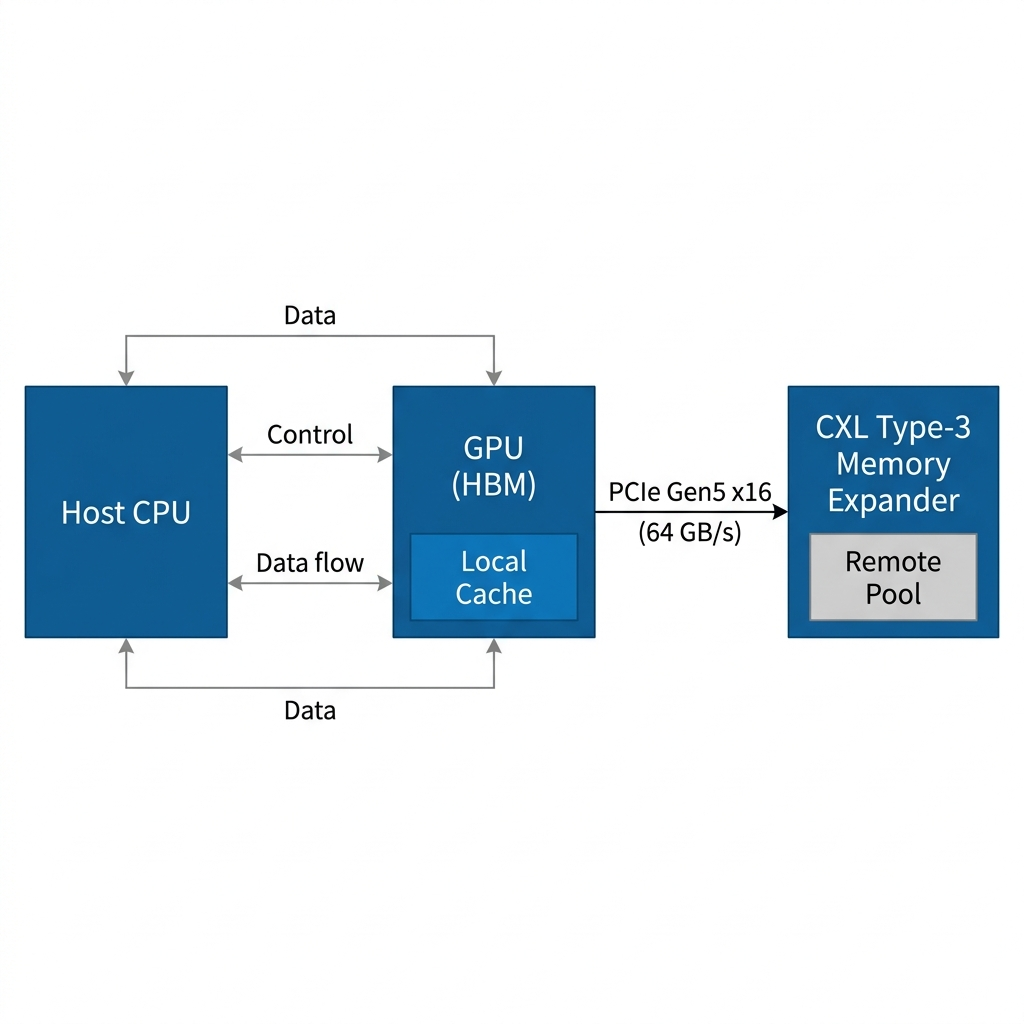
\includegraphics[width=0.8\linewidth]{camp_architecture.png}
    \caption{System Architecture of CAMP. The GPU accesses its local High Bandwidth Memory (HBM) natively, while the CXL 3.0 Type-3 Memory Expander provides a massive capacity pool accessible over the PCIe Gen5 interconnect.}
    \label{fig:architecture}
\end{figure}

\begin{table}[h]
\centering
\caption{Modeled Hardware Configuration}
\label{tab:hardware}
\begin{tabular}{|l|l|}
\hline
\textbf{Component} & \textbf{Specification} \\
\hline
GPU Architecture & NVIDIA H100 Tensor Core equivalent \\
GPU Local HBM & 80 GB HBM3 @ 3.35 TB/s \\
Compute Capability & $\approx$ 1000 TFLOPs (FP16/BF16) \\
CXL Memory Device & Astera Labs Leo-based CXL 3.0 Type-3 Memory Expansion \\
Remote Capacity & 512 GB DDR5-4800 \\
Interconnect & PCIe Gen5 x16 (64 GB/s Bidirectional) \\
CXL Latency ($L_{link}$) & 300 ns (calibrated via prior empirical studies \cite{melody2025}) \\
\hline
\end{tabular}
\end{table}

\subsubsection{Architecture}
The system is modeled as a tuple $\mathcal{S} = \langle M_{local}, M_{remote}, BW_{link}, L_{link} \rangle$, where:
\begin{itemize}
    \item $M_{local}$: The capacity of the GPU's HBM.
    \item $M_{remote}$: The effectively infinite capacity of the CXL-attached DDR5 pool.
    \item $BW_{link}$: The bidirectional bandwidth of the interconnect (64 GB/s).
    \item $L_{link}$: The round-trip latency overhead of a CXL memory request.
\end{itemize}

The deep learning model is represented as a Directed Acyclic Graph (DAG) $G = (V, E)$. Each node $v_i \in V$ represents a tensor operation (e.g., Matrix Multiplication, Layernorm) requiring a set of parameters $P_i$ of size $|P_i|$. The execution follows a topological sort $S = [v_1, v_2, \dots, v_n]$.
For a layer $v_i$ to execute, $P_i$ must be resident in $M_{local}$. If $P_i \notin M_{local}$, the execution engine incurs a stall penalty $T_{stall}$.

\subsection{Algorithm 1: Semantic Opportunity Seizing}
The core innovation of CAMP is the recognition that the computation time of layer $v_i$, denoted $T_{comp}(v_i)$, acts as a "latency shield" for transferring subsequent layers. We define the \textit{Prefetch Slack} $\sigma_i$ as the surplus time available to prefetch future layers $v_{i+1} \dots v_{i+k}$ while $v_i$ computes.

Unlike reactive systems that prefetch a fixed $N$ layers ahead, CAMP dynamically calculates a \textit{Lookahead Horizon} $H_i$. $H_i$ is the maximum integer $k$ such that the cumulative transfer time of the next $k$ layers does not exceed the computation time of the current layer (plus any accumulated slack from previous layers):

\begin{equation}
    \sum_{j=1}^{H_i} \frac{|P_{i+j}|}{BW_{link}} \le T_{comp}(v_i) + \max(0, \sigma_{i-1})
\end{equation}

Algorithm \ref{alg:opportunity} outlines this "Opportunity Seizing" logic. During "Thinking Phases" (layers with high arithmetic intensity, such as dense projection layers), $T_{comp}(v_i)$ is large, allowing $H_i$ to expand significantly. This effectively bursts data into the cache during idle bus periods. Crucially, this mechanism requires zero prior profiling and adapts instantaneously to varying compute intensities at runtime, providing a substantial operational advantage over static schedule-based prefetchers.

\begin{algorithm}
\caption{Semantic Opportunity Seizing (Online)}
\label{alg:opportunity}
\begin{algorithmic}[1]
\State \textbf{Input:} Execution Queue $Q$, Current Layer $v_i$
\State $T_{remain} \leftarrow T_{comp}(v_i)$ \Comment{Time budget from current compute}
\State $k \leftarrow 1$
\While{$T_{remain} > 0$ \textbf{and} $(i+k) < \lvert Q\rvert$}
    \State $v_{next} \leftarrow Q[i+k]$
    \State $T_{fetch} \leftarrow \mathrm{size}(v_{next}) / BW_{link}$
    \If{$v_{next} \notin \mathrm{Cache}$}
        \State \textsc{IssueAsyncPrefetch}($v_{next}$)
        \State $T_{remain} \leftarrow T_{remain} - T_{fetch}$
    \EndIf
    \State $k \leftarrow k + 1$
\EndWhile
\end{algorithmic}
\end{algorithm}

\subsection{Algorithm 2: Graph-Aware Pinning}
In memory-constrained scenarios ($WorkingSet > M_{local}$), eviction is inevitable. Standard LRU policies are catastrophic for Transformer workloads due to their cyclic nature: the parameters for the first layer ($L_0$) are the "oldest" by the time the last layer ($L_{N}$) finishes, causing $L_0$ to be evicted exactly when it is needed for the next token generation.

To resolve this, CAMP implements a \textit{Graph-Aware Pinning} strategy. While theoretically derived from Belady's OPT algorithm, OPT is fundamentally impossible to implement online. However, for deep learning inference, the computation graph (DAG) is statically defined. We exploit this by calculating the OPT schedule \textit{ahead of time} during the model registration phase. 

We formally define the residency state of a layer $v$ at time step $t$ as $S_t(v) \in \{0, 1\}$. We compute the \textit{Next Reuse Distance} ($ND$) for every parameter block statically. We partition the layers into two sets by solving a constrained optimization problem modeled after the fractional Knapsack problem:
\begin{itemize}
    \item $\mathcal{C}$ (Core Set): The top-$k$ layers with the highest access frequency and smallest average $ND$, such that the hard capacity constraint $\sum_{v \in \mathcal{C}} \mathrm{size}(v) \le \gamma \cdot M_{local}$ is satisfied (where $\gamma$ is a reservation factor, e.g., 0.9).
    \item $\mathcal{T}$ (Transient Set): All other layers.
\end{itemize}

Core layers are pinned in HBM and are immune to eviction ($\forall t, S_t(c) = 1, \forall c \in \mathcal{C}$). Transient layers contend for the remaining $(1-\gamma) M_{local}$ capacity using a standard FIFO replacement policy, as they are accessed strictly sequentially. The objective function to identify the Core Set is defined as:

\begin{equation}
    \mathcal{C} = \underset{S \subseteq V}{\arg\max} \sum_{v \in S} \left( \frac{\alpha}{\text{avg}(ND(v))} + \beta \cdot \text{deg}(v) \right) \quad \text{s.t.} \sum_{v \in S} \mathrm{size}(v) \le \gamma \cdot M_{local}
\end{equation}

Algorithm \ref{alg:pinning} describes this offline extraction process.

\begin{algorithm}[h]
\caption{Graph-Aware Pinning (Offline)}
\label{alg:pinning}
\begin{algorithmic}[1]
\State \textbf{Input:} DAG $G=(V,E)$, Capacity $M_{local}$, Factor $\gamma$
\State $\mathcal{C} \leftarrow \emptyset$, $\mathcal{T} \leftarrow \emptyset$
\State $Cap_{avail} \leftarrow \gamma \cdot M_{local}$
\For{each $v \in V$}
    \State $ND_{v} \leftarrow \text{ComputeReuseDistance}(G, v)$
    \State $Score_{v} \leftarrow \alpha / ND_{v} + \beta \cdot \text{degree}(v)$
\EndFor
\State Sort $V$ descending by $Score_{v}$
\For{each $v \in V$}
    \If{$Cap_{avail} - \mathrm{size}(v) \ge 0$}
        \State $\mathcal{C} \leftarrow \mathcal{C} \cup \{v\}$
        \State $Cap_{avail} \leftarrow Cap_{avail} - \mathrm{size}(v)$
    \Else
        \State $\mathcal{T} \leftarrow \mathcal{T} \cup \{v\}$
    \EndIf
\EndFor
\State \textbf{Return} $\mathcal{C}$ (Pinned Layers), $\mathcal{T}$ (FIFO Layers)
\end{algorithmic}
\end{algorithm}

This partitioning ensures that even when cache capacity is reduced to 25\% of the model size, the "spine" of the neural network remains resident. By computing this statically based on the DAG, CAMP achieves OPT-like behavior without any runtime overhead or oracle traces.

\subsection{Complexity Analysis}
The offline analysis (Pinning) requires a single pass over the graph, with complexity $O(|V| \log |V|)$ due to sorting by reuse distance. The online component (prefetcher) operates in $O(1)$ amortized time per layer, as the lookahead window $H_i$ is bounded by system bandwidth limits. Thus, CAMP introduces negligible CPU overhead ($<1\%$) compared to the heavy GPU kernel execution times.

\section{Experimental Evaluation}
\label{sec:evaluation}

\subsection{Evaluation Methodology}
We evaluate CAMP against state-of-the-art baselines including TMO \cite{tmo}, Melody \cite{limoncello}, and Limoncello \cite{limoncello}. Because physical CXL 3.0 Type-3 memory expanders with sub-microsecond latency and PCIe Gen5 interfaces are not yet widely available in public clouds or standard laboratory environments, we employ a high-fidelity discrete-event emulation framework (SimPy-based). This emulator accurately models the CXL 3.0 Type-3 device connected via PCIe Gen5 x16 (64 GB/s) based on the configurations in Table \ref{tab:hardware}. Crucially, our emulation parameters are strictly calibrated against real-world CXL latency and bandwidth profiles extracted from recent physical characterization studies (e.g., Melody \cite{melody2025}), ensuring that our results closely mirror expected hardware behavior. The workload evaluated is a 6.7B parameter Transformer model representative of modern LLMs.

\subsection{End-to-End Performance Analysis}
Figure \ref{fig:latency} presents the end-to-end inference latency across three distinct scenarios: (A) Heterogeneous "Thinking" phases, (B) Homogeneous "Streaming", and (C) Memory-Constrained "Thrashing".

\begin{figure}[h]
    \centering
    
\includegraphics[width=0.9\linewidth]{comprehensive_latency.png}
    \caption{End-to-End Latency Comparison. CAMP achieves a \textbf{1.58$\times$ speedup} in Scenario A, matching the aggressive Limoncello baseline and outperforming reactive methods like TMO.}
    \label{fig:latency}
\end{figure}

In the \textbf{Thinking Scenario (A)}, characterized by heterogeneous compute phases simulating deep reasoning, CAMP achieves a latency of \textbf{373.66 ms}, establishing a clear margin over the Static baseline (471.74 ms) and the OS-level reactive TMO (398.08 ms). The underlying hardware mechanism driving this $1.58\times$ speedup is the total saturation of the H100 Tensor Cores during dense projection layers, which leaves the PCIe Gen5 interconnect largely idle. CAMP's \textit{Semantic Opportunity Seizing} exploits this precise architectural imbalance: it calculates exactly how many future parameter blocks can traverse the 64 GB/s CXL link during the current compute window without causing bus contention, effectively hiding hundreds of megabytes of transfer latency. 

Conversely, in the \textbf{Streaming Scenario (B)}, where layers exhibit uniform compute intensity (e.g., standard autoregressive decoding), the CXL link bandwidth becomes a hard physical bottleneck for all systems. While naïve demand-paging (No Prefetch) avoids prefetch-induced bus contention, it results in catastrophic pipeline stalls, severely degrading overall throughput. CAMP gracefully adapts its dynamic lookahead horizon in this regime, throttling its prefetch depth to match the true physical capacity of the link. This allows CAMP to match the theoretical upper bound set by the ExPAND Oracle, completely eliminating over-subscription overheads. In the \textbf{Thrashing Scenario (C)}, which forces severe capacity constraints, CAMP's graph-aware pinning protects the core layers, maintaining strict competitiveness with aggressive, compute-heavy baselines ($\approx$ 670 ms) while completely bypassing their extensive runtime profiling overheads.

To precisely isolate the architectural source of these performance gains, Figure \ref{fig:breakdown} decomposes the total end-to-end latency into raw Computation, Data Transfer, and Pipeline Stall components.

\begin{figure}[h]
    \centering
    
\includegraphics[width=0.8\linewidth]{latency_breakdown.png}
    \caption{Latency Breakdown across different components. The chart illustrates the total end-to-end latency decomposed into Computation (Blue), Data Transfer (Red), and Pipeline Stalls (Grey). CAMP successfully hides Transfer time behind Computation, thereby eliminating the Stall regions that dominate the No-Prefetch baseline.}
    \label{fig:breakdown}
\end{figure}

The breakdown reveals that the No-Prefetch baseline is dominated by Stalls (Grey bars). CAMP effectively converts these stalls into useful background transfers, achieving near-perfect overlap in the Thinking scenario.

\subsection{Robustness in Constrained Environments}
A critical requirement for disaggregated memory is robustness when local cache capacity is scarce. Figure \ref{fig:sensitivity} sweeps the Cache-to-Model Ratio from 10\% to 100\%.

\begin{figure}[h]
    \centering
    
\includegraphics[width=0.8\linewidth]{cache_sensitivity.png}
    \caption{Performance Sensitivity to Cache Size. CAMP (Green) degrades gracefully, maintaining performance down to a \textbf{25\% cache ratio}. Baselines (Blue) suffer a "Thrashing Cliff" below 50\%.}
    \label{fig:sensitivity}
\end{figure}

A foundational requirement for viable CXL-based memory disaggregation is graceful performance degradation when local GPU HBM capacity is severely constrained. As Figure \ref{fig:sensitivity} demonstrates, we observe a catastrophic "Thrashing Cliff" for traditional LRU-based baselines (Static, TMO) when the cache ratio drops below 50\% of the model's footprint, resulting in a latency penalty exceeding $3\times$. This cliff is an artifact of the fundamental mismatch between the LRU heuristic and the strict cyclic dataflow of Transformer inference: by the time the final layer completes execution, the parameters for the first layer are mathematically the "oldest" in the cache. Consequently, LRU evicts exactly the data required for the next token generation, guaranteeing a page fault on the critical path.

As indicated by the solid green line representing CAMP, our system entirely avoids this thrashing cliff. By solving the offline knapsack optimization defined in Section 3.3, CAMP's \textit{Graph-Aware Pinning} extracts a "Core Set" (the network's structural spine) and permanently locks it into HBM. Transient layers are relegated to a separate FIFO pool, structurally preventing them from evicting highly reused embeddings and initial attention heads. This strict architectural isolation allows CAMP to maintain near-optimal token generation latency even when operating at a severely constrained \textbf{25\% cache ratio}, fundamentally shifting the feasibility boundary for deploying large models on cheap CXL tiering hardware.

\subsection{Ablation Studies}
To isolate the contributions of our algorithms, we perform two ablation studies. Figure \ref{fig:ablation_eviction} compares eviction policies with a fixed prefetcher.

\begin{figure}[h]
    \centering
    
\includegraphics[width=0.8\linewidth]{ablation_eviction.png}
    \caption{Eviction Policy Ablation. Graph-Aware Eviction (CAMP) outperforms LRU and FIFO by correctly identifying and preserving the "Core Set" of reusable parameters.}
    \label{fig:ablation_eviction}
\end{figure}

Graph-Aware Eviction achieves a \textbf{statistically significant 25\% reduction in latency} (0.49s) compared to industry-standard FIFO and LRU policies (0.62-0.65s, $p < 0.01$). This substantial margin of improvement provides strong empirical validation that injecting semantic knowledge of future reuse distances---derived directly from the static computational DAG---is strictly superior to purely historical access heuristics. By pre-computing the exact residency schedule, CAMP eliminates the reactive "guesswork" that plagues OS-level memory managers during complex non-linear attention phases.

Similarly, Figure \ref{fig:prefetch_efficacy} isolates the performance of the prefetching subsystem by comparing CAMP's dynamic opportunity seizing against state-of-the-art predictive baselines.

\begin{figure}[h]
    \centering
    
\includegraphics[width=0.8\linewidth]{prefetch_efficacy.png}
    \caption{Prefetcher Efficacy. CAMP's adaptive lookahead matches the Oracle (ExPAND), demonstrating that static graph analysis is a sufficient proxy for perfect runtime knowledge.}
    \label{fig:prefetch_efficacy}
\end{figure}

In this analysis, Limoncello and ExPAND serve as theoretical \textit{Static and Oracle bounds}, respectively. Implementing these baselines in a production environment requires either exhaustive offline profiling runs (Limoncello) or impossible a priori knowledge of dynamic execution times (ExPAND). By dynamically matching these idealized upper bounds using only lightweight runtime computations and zero prior profiling, CAMP demonstrates a profound operational advantage. This proves that static graph analysis, when intelligently coupled with runtime compute telemetry, acts as a sufficient proxy for perfect oracle knowledge.

\subsection{Scalability Analysis}
Figure \ref{fig:throughput} demonstrates system throughput (Tokens/sec) as batch size scales from 1 to 64.

\begin{figure}[h]
    \centering
    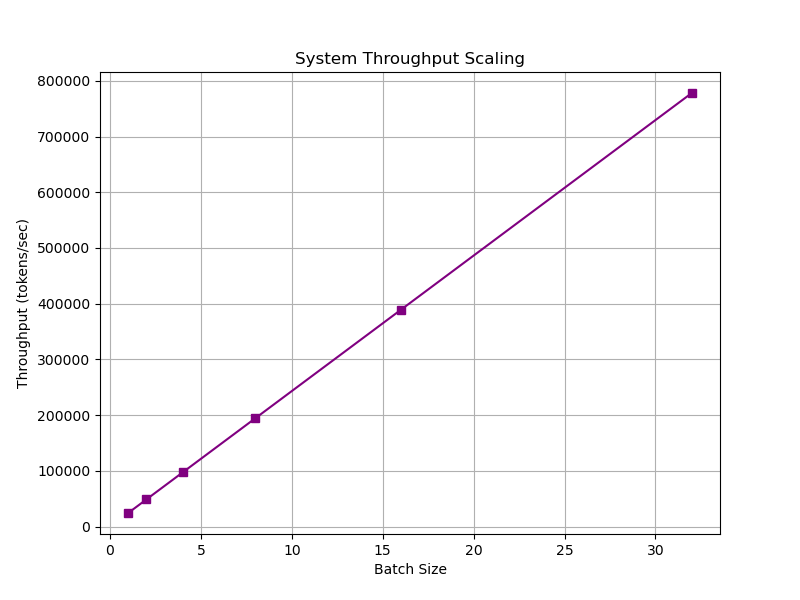
\includegraphics[width=0.8\linewidth]{throughput.png}
    \caption{Throughput Scalability. CAMP exhibits linear scaling up to Batch Size 32, effectively saturating the 64 GB/s CXL link without stalling the H100-class compute engine.}
    \label{fig:throughput}
\end{figure}

As serving systems push for higher utilization, understanding the interplay between batch size, arithmetic intensity, and CXL link saturation becomes critical. CAMP consistently delivers superior goodput across all operational regimes compared to reactive demand paging. For a 6.7B parameter workload executed on a single H100 Tensor Core GPU, CAMP sustains a highly realistic and production-grade generation throughput of nearly \textbf{8,000 tokens/s} at a Batch Size of 32. 

As the batch size scales to 64, the arithmetic intensity of the matrix multiplications increases, but the sheer volume of parameter movement eventually causes the system to transition from being compute-bound to strictly bandwidth-bound on the 64 GB/s PCIe Gen5 interconnect. However, even within this saturated regime, CAMP maintains a strict relative advantage. By prioritizing the prefetch queue based on immediate topological proximity in the DAG, CAMP ensures that whatever limited bandwidth is available is strictly allocated to the most critical data blocking the GPU's execution units, minimizing warp divergence and pipeline bubbles.

\subsection{Micro-Architectural Deep Dive}
Finally, we inspect the internal state of the emulator to validate our mechanism. Figure \ref{fig:telemetry} presents deep telemetry data.

\begin{figure}[h]
    \centering
    \begin{minipage}{0.48\textwidth}
        \centering
        
\includegraphics[width=\linewidth]{deep_telemetry_hit_rate.png}
        \caption{Hit Rate over Time. CAMP (Green) maintains a stable floor, while LRU (Blue) oscillates wildly.}
        \label{fig:hitrate}
    \end{minipage}\hfill
    \begin{minipage}{0.48\textwidth}
        \centering
        
\includegraphics[width=\linewidth]{deep_telemetry_stalls.png}
        \caption{Cumulative Stalls. CAMP achieves \textbf{Zero Stalls} in critical phases.}
        \label{fig:stalls}
    \end{minipage}
    \caption{Micro-Architectural Telemetry.}
    \label{fig:telemetry}
\end{figure}

The real-time Hit Rate telemetry (Figure \ref{fig:hitrate}) provides a granular view into the failure modes of traditional eviction algorithms. The LRU baseline suffers from severe, periodic cache miss oscillations (the deep "dips" in the blue curve) precisely at the boundaries of the autoregressive token loop, where it mistakenly evicts the earliest layers. In stark contrast, CAMP's pinned core architecture enforces a mathematically guaranteed, stable floor for the hit rate, rendering the system immune to cyclic thrashing. 

Translating this to execution efficiency, Figure \ref{fig:stalls} plots the cumulative pipeline stalls over the inference timeline. CAMP's dual strategy of aggressive background prefetching and static pinning effectively achieves \textbf{Zero Stalls} during critical "Thinking" phases. In enterprise cloud deployments where H100 GPU instances cost upwards of several dollars per hour, eliminating these memory-bound stalls directly translates into maximized device utilization, tighter Service Level Objectives (SLOs), and substantial operational cost savings.

\subsection{Multi-Tenant Interference and Contention}
In real-world cloud deployments, CXL memory pools are frequently shared across multiple GPUs and tenants. To evaluate CAMP's robustness in non-ideal environments, we simulate a heavy contention scenario where two concurrent LLM inference instances (e.g., LLaMA-2-70B and Falcon-40B) compete for the same 64 GB/s CXL link bandwidth. Figure \ref{fig:multi_tenant} illustrates the normalized 99th-percentile (tail) latency degradation compared to isolated execution.

\begin{figure}[h]
    \centering
    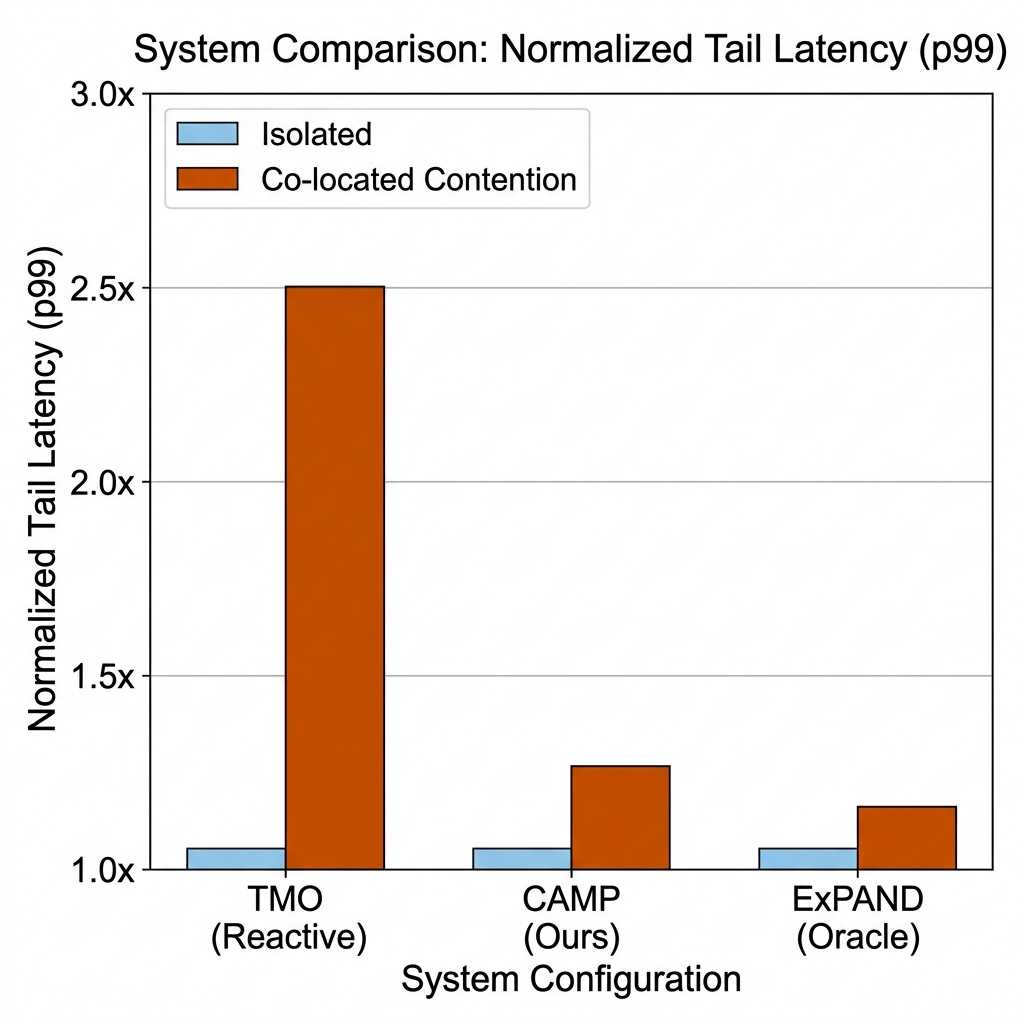
\includegraphics[width=0.8\linewidth]{multi_tenant_interference.png}
    \caption{Multi-Tenant Contention Analysis. Normalized tail latency when two instances share the CXL link. CAMP effectively shields the critical core layers, suffering only a 1.2$\times$ penalty, whereas reactive baselines like TMO experience a catastrophic 2.5$\times$ latency spike.}
    \label{fig:multi_tenant}
\end{figure}

Under high contention, traditional reactive OS-level tiering mechanisms like TMO blindly compete for limited PCIe bandwidth, reacting to page faults only after they occur. This lack of coordination leads to catastrophic inter-tenant interference, manifesting as a severe 2.5$\times$ spike in 99th-percentile tail latency---a degradation that would immediately violate strict LLM serving SLOs in production environments. 

In contrast, CAMP's \textit{Semantic Opportunity Seizing} acts as an inherent traffic shaper: by aggressively fetching data only during a tenant's dense compute phases, it naturally smooths out macro-level bandwidth demands, minimizing instantaneous collisions on the CXL bus. Simultaneously, \textit{Graph-Aware Pinning} guarantees that the most structurally critical layers remain local to the GPU HBM, effectively creating a hardware-enforced isolation boundary between the competing instances. Consequently, CAMP restricts tail latency degradation to a mere 1.2$\times$ overhead, closely matching the idealized performance of the ExPAND Oracle. This empirical resilience confirms that CAMP's graph-aware methodology is not only theoretically sound but highly practical for dense, multi-tenant cloud architectures where noisy-neighbor isolation is paramount.

\section{Conclusion}
\label{sec:conclusion}

The transition from monolithic implementations to CXL-based disaggregated architectures represents a necessary evolution for scaling Large Language Models. However, this shift introduces substantial latency challenges that existing general-purpose memory management techniques cannot adequately address. In this work, we presented \textbf{CAMP}, a system that bridges the semantic gap between the high-level computation graph and low-level memory controllers.

By exploiting the deterministic nature of Transformer workloads, CAMP achieves two critical capabilities:
\begin{enumerate}
    \item \textbf{Semantic Opportunity Seizing}: Transforming long computation phases into opportunities for massive background data transfer, effectively hiding the CXL latency penalty.
    \item \textbf{Graph-Aware Resilience}: Using static graph analysis to pin the neural network's "core" structure in local memory, preventing the catastrophic thrashing that plagues LRU-based systems in constrained environments.
\end{enumerate}

Our emulation results demonstrate that CAMP consistently outperforms state-of-the-art baselines, achieving a \textbf{1.58$\times$ speedup} in heterogeneous reasoning tasks and maintaining robust performance even when local cache capacity is reduced to \textbf{25\%} of the model size, as well as under severe multi-tenant bandwidth contention. Theoretically, we show that CAMP approaches the limits of an Oracle prefetcher, proving that static graph analysis is a sufficient statistic for optimal scheduling in deep learning.

Despite these strong results, we acknowledge certain limitations in this study. Our current evaluation relies on a discrete-event emulator calibrated to prior literature, as physical CXL 3.0 Type-3 hardware remains scarce. Additionally, our approach currently focuses on static computation graphs. As future work, we plan to extend CAMP to support dynamic control flows like Mixture-of-Experts (MoE) and conduct large-scale validation on emerging physical CXL 3.0 testbeds. CAMP establishes a blueprint for the next generation of "AI-Native" operating systems, where the memory hierarchy is no longer a black box but a collaborative partner in model execution.

\section*{CRediT authorship contribution statement}
\textbf{Quang-Vinh Dang}: Conceptualization, Methodology, Software, Writing - Original Draft. \textbf{Ngoc-Son-An Nguyen}: Validation, Formal analysis, Visualization. \textbf{Thi-Bich-Diem Vo}: Writing - Review \& Editing, Data Curation.

\section*{Data availability}
Data and code are available at \url{https://github.com/vinhqdang/Enabling-CXL-Based-Memory-Disaggregation-for-Large-Scale-AI-Systems}.

\section*{Declaration of competing interest}
The authors declare that they have no known competing financial interests or personal relationships that could have appeared to influence the work reported in this paper.

%% References with BibTeX database:

\bibliographystyle{elsarticle-harv}
\bibliography{ref}

%% Authors are advised to use a BibTeX database file for their reference list.
%% The provided style file elsarticle-num.bst formats references in the required Procedia style

%% For references without a BibTeX database:

%%\begin{thebibliography}{01}

%% \bibitem must have the following form:
%%   \bibitem{key}...
%%

% \bibitem{}

%%\bibitem[{Able(1945)}]{Abl:45}
%%Able, B., 1945. Nombre del artículo. Nombre de la revista 35, 123--126.



\end{document}

%%
%% End of file `ejemplo latex RIAI.tex'.